\documentclass[10pt,a4paper,oneside,fleqn]{article}
\usepackage{geometry}
\geometry{a4paper,left=20mm,right=20mm,top=1cm,bottom=2cm}
\usepackage[utf8]{inputenc}
%\usepackage{ngerman}
\usepackage{amsmath}                % brauche ich um dir Formel zu umrahmen.
\usepackage{amsfonts}                % brauche ich für die Mengensymbole
\usepackage{graphicx}
\setlength{\parindent}{0px}
\setlength{\mathindent}{10mm}
\usepackage{bbold}                    %brauche ich für die doppel Zahlen Darstellung (Einheitsmatrix z.B)
\usepackage{dsfont}          %F�r den Einheitsoperator \mathds 1


\usepackage{color}
\usepackage{titlesec} %sudo apt-get install texlive-latex-extra

\definecolor{darkblue}{rgb}{0.1,0.1,0.55}
\definecolor{verydarkblue}{rgb}{0.1,0.1,0.35}
\definecolor{darkred}{rgb}{0.55,0.2,0.2}

%hyperref Link color
\usepackage[colorlinks=true,
        linkcolor=darkblue,
        citecolor=darkblue,
        filecolor=darkblue,
        pagecolor=darkblue,
        urlcolor=darkblue,
        bookmarks=true,
        bookmarksopen=true,
        bookmarksopenlevel=3,
        plainpages=false,
        pdfpagelabels=true]{hyperref}

\titleformat{\chapter}[display]{\color{darkred}\normalfont\huge\bfseries}{\chaptertitlename\
\thechapter}{20pt}{\Huge}

\titleformat{\section}{\color{darkblue}\normalfont\Large\bfseries}{\thesection}{1em}{}
\titleformat{\subsection}{\color{verydarkblue}\normalfont\large\bfseries}{\thesubsection}{1em}{}

% Notiz Box
\usepackage{fancybox}
\newcommand{\notiz}[1]{\vspace{5mm}\ovalbox{\begin{minipage}{1\textwidth}#1\end{minipage}}\vspace{5mm}}

\usepackage{cancel}
\setcounter{secnumdepth}{3}
\setcounter{tocdepth}{3}





%-------------------------------------------------------------------------------
%Diff-Makro:
%Das Diff-Makro stellt einen Differentialoperator da.
%
%Benutzung:
% \diff  ->  d
% \diff f  ->  df
% \diff^2 f  ->  d^2 f
% \diff_x  ->  d/dx
% \diff^2_x  ->  d^2/dx^2
% \diff f_x  ->  df/dx
% \diff^2 f_x  ->  d^2f/dx^2
% \diff^2{f(x^5)}_x  ->  d^2(f(x^5))/dx^2
%
%Ersetzt man \diff durch \pdiff, so wird der partieller
%Differentialoperator dargestellt.
%
\makeatletter
\def\diff@n^#1{\@ifnextchar{_}{\diff@n@d^#1}{\diff@n@fun^#1}}
\def\diff@n@d^#1_#2{\frac{\textrm{d}^#1}{\textrm{d}#2^#1}}
\def\diff@n@fun^#1#2{\@ifnextchar{_}{\diff@n@fun@d^#1#2}{\textrm{d}^#1#2}}
\def\diff@n@fun@d^#1#2_#3{\frac{\textrm{d}^#1 #2}{\textrm{d}#3^#1}}
\def\diff@one@d_#1{\frac{\textrm{d}}{\textrm{d}#1}}
\def\diff@one@fun#1{\@ifnextchar{_}{\diff@one@fun@d #1}{\textrm{d}#1}}
\def\diff@one@fun@d#1_#2{\frac{\textrm{d}#1}{\textrm{d}#2}}
\newcommand*{\diff}{\@ifnextchar{^}{\diff@n}
  {\@ifnextchar{_}{\diff@one@d}{\diff@one@fun}}}
%
%Partieller Diff-Operator.
\def\pdiff@n^#1{\@ifnextchar{_}{\pdiff@n@d^#1}{\pdiff@n@fun^#1}}
\def\pdiff@n@d^#1_#2{\frac{\partial^#1}{\partial#2^#1}}
\def\pdiff@n@fun^#1#2{\@ifnextchar{_}{\pdiff@n@fun@d^#1#2}{\partial^#1#2}}
\def\pdiff@n@fun@d^#1#2_#3{\frac{\partial^#1 #2}{\partial#3^#1}}
\def\pdiff@one@d_#1{\frac{\partial}{\partial #1}}
\def\pdiff@one@fun#1{\@ifnextchar{_}{\pdiff@one@fun@d #1}{\partial#1}}
\def\pdiff@one@fun@d#1_#2{\frac{\partial#1}{\partial#2}}
\newcommand*{\pdiff}{\@ifnextchar{^}{\pdiff@n}
  {\@ifnextchar{_}{\pdiff@one@d}{\pdiff@one@fun}}}
\makeatother
%
%Das gleich nur mit etwas andere Syntax. Die Potenz der Differentiation wird erst
%zum Schluss angegeben. Somit lautet die Syntax:
%
% \diff_x^2  ->  d^2/dx^2
% \diff f_x^2  ->  d^2f/dx^2
% \diff{f(x^5)}_x^2  ->  d^2(f(x^5))/dx^2
% Ansonsten wie Oben.
%
%Ersetzt man \diff durch \pdiff, so wird der partieller
%Differentialoperator dargestellt.
%
%\makeatletter
%\def\diff@#1{\@ifnextchar{_}{\diff@fun#1}{\textrm{d} #1}}
%\def\diff@one_#1{\@ifnextchar{^}{\diff@n{#1}}%
%  {\frac{\textrm d}{\textrm{d} #1}}}
%\def\diff@fun#1_#2{\@ifnextchar{^}{\diff@fun@n#1_#2}%
%  {\frac{\textrm d #1}{\textrm{d} #2}}}
%\def\diff@n#1^#2{\frac{\textrm d^#2}{\textrm{d}#1^#2}}
%\def\diff@fun@n#1_#2^#3{\frac{\textrm d^#3 #1}%
%  {\textrm{d}#2^#3}}
%\def\diff{\@ifnextchar{_}{\diff@one}{\diff@}}
%\newcommand*{\diff}{\@ifnextchar{_}{\diff@one}{\diff@}}
%
%Partieller Diff-Operator.
%\def\pdiff@#1{\@ifnextchar{_}{\pdiff@fun#1}{\partial #1}}
%\def\pdiff@one_#1{\@ifnextchar{^}{\pdiff@n{#1}}%
%  {\frac{\partial}{\partial #1}}}
%\def\pdiff@fun#1_#2{\@ifnextchar{^}{\pdiff@fun@n#1_#2}%
%  {\frac{\partial #1}{\partial #2}}}
%\def\pdiff@n#1^#2{\frac{\partial^#2}{\partial #1^#2}}
%\def\pdiff@fun@n#1_#2^#3{\frac{\partial^#3 #1}%
%  {\partial #2^#3}}
%\newcommand*{\pdiff}{\@ifnextchar{_}{\pdiff@one}{\pdiff@}}
%\makeatother

%-------------------------------------------------------------------------------
%%Nützliche Makros um in der Quantenmechanik Bras, Kets und das Skalarprodukt
%%zwischen den beiden darzustellen.
%%Benutzung:
%% \bra{x}  ->    < x |
%% \ket{x}  ->    | x >
%% \braket{x}{y} ->   < x | y >



\newcommand\bra[1]{\left\langle #1 \right|}
\newcommand\ket[1]{\left| #1 \right\rangle}
\newcommand\braket[2]{%
 \left\langle \vphantom{#2} #1%
   \middle|%
   \vphantom{#1} #2\right\rangle}%

%-------------------------------------------------------------------------------
%%Aus dem Buch:
%%Titel:  Latex in Naturwissenschaften und Mathematik
%%Autor:  Herbert Voß
%%Verlag: Franzis Verlag, 2006
%%ISBN:   3772374190, 9783772374197
%%
%%Hier werden drei Makros definiert:\mathllap, \mathclap und \mathrlap, welche
%%analog zu den aus Latex bekannten \rlap und \llap arbeiten, d.h. selbst
%%keinerlei horizontalen Platz benötigen, aber dennoch zentriert zum aktuellen
%%Punkt erscheinen.

\newcommand*\mathllap{\mathstrut\mathpalette\mathllapinternal}
\newcommand*\mathllapinternal[2]{\llap{$\mathsurround=0pt#1{#2}$}}
\newcommand*\clap[1]{\hbox to 0pt{\hss#1\hss}}
\newcommand*\mathclap{\mathpalette\mathclapinternal}
\newcommand*\mathclapinternal[2]{\clap{$\mathsurround=0pt#1{#2}$}}
\newcommand*\mathrlap{\mathpalette\mathrlapinternal}
\newcommand*\mathrlapinternal[2]{\rlap{$\mathsurround=0pt#1{#2}$}}

%%Das Gleiche nur mit \def statt \newcommand.
%\def\mathllap{\mathpalette\mathllapinternal}
%\def\mathllapinternal#1#2{%
%  \llap{$\mathsurround=0pt#1{#2}$}% $
%}
%\def\clap#1{\hbox to 0pt{\hss#1\hss}}
%\def\mathclap{\mathpalette\mathclapinternal}
%\def\mathclapinternal#1#2{%
%  \clap{$\mathsurround=0pt#1{#2}$}%
%}
%\def\mathrlap{\mathpalette\mathrlapinternal}
%\def\mathrlapinternal#1#2{%
%  \rlap{$\mathsurround=0pt#1{#2}$}% $
%}

%-------------------------------------------------------------------------------
%%Hier werden zwei neue Makros definiert \overbr und \underbr welche analog zu
%%\overbrace und \underbrace funktionieren jedoch die Gleichung nicht
%%'zerreißen'. Dies wird ermöglicht durch das \mathclap Makro.

\def\overbr#1^#2{\overbrace{#1}^{\mathclap{#2}}}
\def\underbr#1_#2{\underbrace{#1}_{\mathclap{#2}}}


\begin{document}
\tableofcontents
\setcounter{chapter}{5}
\chapter{Relativistische QM}



Notation: Vierer-Vektoren

\[x^{\mu} = (ct,x,y,z) = (x^0,x^1,x^2,x^3) = (ct,\vec r)\]

invariante Länge \(\sqrt{x^2}\)

\[x^2=x\cdot x = x^{\mu}x_\mu = x^\mu g_{\mu \nu}x^\nu\]

Einsteinsche Summenkonvention: \(\sum_{\mu=0}^3\) für jedes Paar von oberen und unteren Index

\underline{Metrischer Tensor}

\[ g_{\mu\nu} = \begin{bmatrix}
 1 & 0 & 0 & 0\\
 0 & -1 & 0 & 0\\
 0 & 0 & -1 & 0\\
 0 & 0 & 0 & -1\\
\end{bmatrix} \]

\[ x_\mu = g_{\mu\nu}x^\nu = (ct,-\vec r)\]

\[x^\mu = g^{\mu\nu}x_\nu = g^{\mu\nu}x^\nu = g^\nu_{\,\,\nu} x^\nu\] 

\[g^\nu_{\,\,\nu} = \delta^\nu{\,\,_\nu} =\begin{cases}
  1,  & \mu = \nu\\
  0 & \text{sonst}
\end{cases} \]

\[= g^{\mu\rho}g_{\rho\nu} \rightarrow  g^{\mu\nu} = [g_{\mu\nu}]^{-1} = \begin{bmatrix}
 1 & 0 & 0 & 0\\
 0 & -1 & 0 & 0\\
 0 & 0 & -1 & 0\\
 0 & 0 & 0 & -1\\
\end{bmatrix} \]

\underline{Vierer-Impuls}: \(p^\mu=(\frac{E}{c},\vec p)\)  mit  \(E= \sqrt{(mc^2)^2+(\vec p c)^2}\)

\[p^2 = p_\mu p^\mu = \frac{E^2}{c^2}-\vec p^2 = \frac{m^2c^4+\vec p^2 c^2}{c^2} - \vec p^2 = m^2c^2\]

\underline{Vierer-Potential}:  Lorenz-Transformation \(x^{'\mu} = \Lambda^{\mu}_{\,\,\nu} x^\nu\)

\[A^\mu = (\frac{\phi}{c},\vec A) \qquad \rightarrow  A^{'\mu}(x') = \Lambda^\mu_{\,\,\nu} A^\nu(x)\]

\underline{Strom}: \(j^\mu = (c\rho,\vec j)\) in E und M

Skalarprodukt für \(a^\mu,b^\mu: \qquad a\cdot b = a^\mu b_\mu = a^\mu g_{\mu\nu}b^\nu = a^0 b^0 - \vec a\cdot \vec b\)

Ableitung nach \(x^\nu\)

\[\partial_\mu = \frac{\partial}{\partial x^\mu} = (\frac{1}{c} \frac{\partial}{\partial t},\vec \nabla )\]

ist kovarianter Vektor (Index unten) wegen: \(\partial_{\mu} a\cdot x = \frac{\partial}{\partial x^\mu}(a_\nu x^\nu)= a_\mu\)

Entsprechend \(\partial^\mu = g^{\mu\nu}\partial_\nu = (\frac{1}{c}\frac{\partial}{\partial t},-\vec\nabla)\)


d'Alebert Operator

\[\square = \partial_\mu\partial^\mu = \frac{1}{c^2} \frac{\partial^2}{\partial t^2} - \vec \nabla^2\]



\subsection{QM eines freien Teilchens}

\[E\rightarrow i\hbar\frac{\partial}{\partial t}, \quad \vec p = \frac{\hbar}{i}\vec \nabla\]

\[ p^\mu = (\frac{E}{c},\vec p) \rightarrow (i\hbar \frac{1}{c}\frac{\partial}{\partial t},-i\hbar \vec \nabla) = i\hbar\partial^\mu\]

Schrödinger Gl. für nicht relativistisches freies Teilchen (ohne Potential)

\[E=\frac{\vec p^2}{2m} \rightarrow  i\hbar \frac{\partial }{\partial t}\psi = -\frac{\hbar^2\nabla^2}{2m}\psi(\vec x,t) \]


Relativistischer Fall


\begin{enumerate}
\item[1)] \(E = \sqrt{m^2c^4+\vec p^2c^2} \rightarrow \) nichtlokaler Operator
\item[2)] \(\frac{E^2}{c^2} = m^2c^2 + \vec p^2 \rightarrow - \frac{\hbar^2}{c^2}\frac{\partial^2 }{\partial t^2}\psi = m^2c^2\psi -\hbar^2\vec \nabla^2\psi \)
\end{enumerate}

\[ - \frac{\hbar^2}{c^2}\frac{\partial^2 }{\partial t^2}\psi = m^2c^2\psi -\hbar^2\vec \nabla^2\psi\]
\begin{align}
\Leftrightarrow  0 &= m^2c^2\psi + \hbar^2\left(\frac{1}{c^2}\frac{\partial^2}{\partial t^2}  - \nabla^2\right)\psi\\
0&= m^2c^2\psi+\hbar^2 \square \psi
\end{align}


\underline{Klein Gordon} Gleichung:

\[\boxed{\left(\square + \left(\frac{mc}{\hbar}\right)^2\right)\psi(x) = 0}\]

Anwendbar auf skalare Teilichen (Spin 0) wie \(\pi^+,\pi^-,\pi^0,K,H\)

Lösungen der KG-Gl. durch ebene Wellen

\[\psi_p(x) = N e^{-ip\cdot x/\hbar} = Ne^{-iEt/\hbar}e^{+i\vec p\cdot\vec x/\hbar}\]

mit \(p\cdot x = p^\mu x_\mu = Et-\vec p\cdot \vec x\)

\[\square \psi_p (x) = \frac{\partial}{\partial x^\mu} \frac{\partial}{\partial x_\mu} \psi_p(x) = N(-\frac{i}{\hbar}p_\mu)(-\frac{i}{\hbar}p^\mu) e^{-ip\cdot x/\hbar} = -\frac{p^2}{\hbar^2}\psi_p \]


Klein Gordon Gleichung:

\[\Rightarrow \left(-\frac{p^2}{\hbar^2} + \frac{m^2c^2}{\hbar^2}\right)\psi_p(x) = 0\]

\[ \Leftrightarrow p^2 = m^2 c^2 = \frac{E^2}{c^2}-\vec p^2\]

\[\rightarrow E = \pm c \sqrt{m^2c^2+\vec p^2}\]


Lösungen mit Negativer Energie und das Energiespektrum ist nach unten nicht beschränkt. 



\subsection{Wahrscheinlichkeitserhaltung}

Kontinuitäts-Gleichung

 \[\frac{\partial\rho}{\partial t}+\vec \nabla\cdot \vec j = 0 \Leftrightarrow \partial_\mu j^\mu = 0\]

mit \(j^\mu = (\rho c,\vec j)\) und \(\partial_\mu = (\frac{1}{c} \frac{\partial}{\partial t},\vec \nabla )\). 


Gibt es einen erhaltenen 4-Strom für die lösung der Klein-Gordon-Gleichung?

\[\psi^*(\square + (\frac{mc}{\hbar})^2)\psi(x) - \psi(\square + (\frac{mc}{\hbar})^2)\psi^*(x) = 0\]

\[\psi^*\square\psi(x) + \psi^*(x)(\frac{mc}{\hbar})^2\psi(x) - \psi\square\psi^*(x) - \psi(x)(\frac{mc}{\hbar})^2\psi^*(x) = 0\]

\[\psi^*\square\psi(x) -  \psi\square\psi^*(x) + \cancel{|\psi(x)|^2(\frac{mc}{\hbar})^2} -\cancel{|\psi(x)|^2(\frac{mc}{\hbar})^2} = 0\]

mit \(\square \psi = \frac{\partial}{\partial x^\mu} \frac{\partial}{\partial x_\mu} \psi\)


\[\psi^*(\partial_\mu\partial^\mu \psi) - \psi(\partial_\mu\partial^\mu \psi^*) = 0 \]

\[\partial_\mu(\underbrace{\psi^*\partial^\mu\psi - \psi \partial^\mu \psi^*}_{\propto j^\mu}) = 0\]

\[ j^\mu \propto (\psi^*\frac{i}{c}\frac{\partial}{\partial t}\psi - \psi\frac{i}{c}\frac{\partial}{\partial t}\psi^* ,-(\psi^*\vec \nabla \psi - \psi\vec \nabla\psi^*)) \]

Kandidat für Wahrscheinlichkeits Strom \(\frac{2im}{\hbar}\vec j\) in Schrödinger Gl

\[j^\mu = \frac{i\hbar}{2m} (\psi^*\partial^\mu \psi - \psi \partial^\mu \psi^*)\]

\[\rightarrow j^0 = \rho c =  \frac{i\hbar}{2mc}(\psi^*\frac{\partial\psi}{\partial t} - \psi\frac{\partial\psi^*}{\partial t}) \]

Anwendung auf stationäre Lösung: \(\psi_E(x) = e^{-iEt/\hbar}\psi_E(\vec x)\)

\[\frac{\partial \psi_E}{\partial t} = -\frac{iE}{\hbar}\psi_E,\frac{\partial \psi_E^*}{\partial t} = \frac{iE}{\hbar}\psi_E^*\]

\begin{align}
\rho &=  \frac{i\hbar}{2mc^2}(\psi^*_E\frac{\partial\psi_E}{\partial t} - \psi_E\frac{\partial\psi^*_E}{\partial t}) \\
&=  \frac{i\hbar}{2mc^2}(-\psi^*_E\frac{iE}{\hbar}\psi_E  - \psi_E \frac{iE}{\hbar}\psi_E^*) \\
&= \frac{i\hbar}{2mc^2}|\psi_E(\vec x)|^2\frac{-2iE}{\hbar}\\
&= \frac{E}{mc^2}|\psi_E(x)|^2
\end{align}

\[ \Rightarrow \boxed{ \rho = \frac{E}{mc^2}|\psi_E(x)|^2} \]

\(\rho < 0\) für Zustände mit \(E<0\)

\(\Rightarrow  \) Keine mögliche Wahrscheinlichkeitsdichte. (Ok für Zustände mit positiver Energie)


\underline{Interpretation}: Zustände mit \(E>0\Leftrightarrow \) z.B. \(\pi^+\) und  \(E<0\Leftrightarrow \) z.B. \(\pi^-\)(Antiteilchen zum  \(\pi^+\))\\
\\
\(\rho > 0\): \(\pi^+\) dominieren
\(\rho < 0\): \(\pi^-\) dominieren\\
\\
\(\rho \propto\) elektromagn. Ladungsdichte

\[ j^\mu = |e|\frac{i\hbar}{2mc} (\psi^*\partial^\mu\psi -\psi\partial^\mu\psi^* )\]


Elektronen: Spin

\(\rightarrow \) Wellenfunktion \(\psi(x)\) hat \(\geq 2\) Komponenten

\[\psi(x) =\begin{pmatrix} \psi_1(x)\\ ...\\ \psi_N(x) \end{pmatrix} \]

Möglichkeit: Matrixstruktur für \(\hat H\)

\[i\hbar \frac{\partial}{\partial t}\psi(x) = \hat H \psi(x)\]




Ansatz: \(i\hbar \frac{\partial }{\partial t} \psi = \hat H \psi\) mit \(\psi(x) =\begin{pmatrix} \psi_1(x)\\ ...\\ \psi_N(x) \end{pmatrix} \)

und Wahrscheinlichkeitsdichte \(\rho = \sum_{i=1}^N |\psi_i|^2\)

\[\Rightarrow \hat H \propto \frac{\partial}{\partial x^i}\propto \hat p_i\]

Ansatz für \(\hat H\)

\[\hat H = c(\alpha_x\hat p_x+\alpha_y\hat p_y+\alpha_z\hat p_z) +\beta mc^2 = c\sum_{i=1}^3 \alpha_i\hat p_i+ \beta mc^2\]

Ebene Wellenlösung für freie Teilchen

\[\psi(x) = e^{-px/\hbar}\psi(p)\]

mit \(p^2 = m^2c^2\)

\[\Rightarrow  E\psi(p) =[c \sum_{i=1}^3 \alpha_ip_i+\beta mc^2]\psi(p)\]

\begin{align}
E^2\psi(p) &=E\cdot [c \sum_{i=1}^3 \alpha_ip_i+\beta mc^2]\psi(p)\\
&=[c \sum_{j=1}^3 \alpha_jp_j+\beta mc^2] \cdot [c \sum_{i=1}^3 \alpha_ip_i+\beta mc^2]\psi(p) \\
&=c^2 [ \sum_{j=1}^3 \alpha_jp_j+\beta mc] \cdot [ \sum_{i=1}^3 \alpha_ip_i+\beta mc]\psi(p) \\
&=c^2 \left( \sum_{j=1}^3 \alpha_jp_j\sum_{i=1}^3 \alpha_ip_i  +   \sum_{j=1}^3 \alpha_jp_j \beta mc  + \beta mc \sum_{i=1}^3 \alpha_ip_i+ \beta^2 m^2c^2\right)\psi(p) \\
&= c^2\left(\sum_{i,j=1}^3\alpha_i\alpha_j p_ip_j+\sum_{i=1}^3(\alpha_i\beta+\beta\alpha_i)p_i mc +  \beta^2m^2c^2\right)\psi(p)\\
&\stackrel{\mathrm{!}}= c^2 (m^2c^2+\vec p^2 )\psi(p)
\end{align}



Koeffizienfenvergleich:
\begin{itemize}
\item  \(\boxed{\beta^2=1}\)
\item Antikommutator: \(\boxed{\{\alpha_i,\beta\}=0}\)
\item \(i\neq j\): z.B: \(p_xp_y\{\alpha_x\alpha_y+\alpha_y\alpha_x\}\); \(\{\alpha_i,\alpha_j\}=0\)
\item \(i=j\): \(\alpha_x^2p_x^2+\alpha_y^2p_y^2+\alpha_z^2p_z^2=\vec p^2 \Rightarrow \alpha_i^2 = 1\)
\[\Rightarrow \boxed{\{\alpha_i,\alpha_j\}=2\delta_{ij}}\]
\end{itemize}


\begin{enumerate}
\item[1)] \(\hat p_i,\hat H\) hermitesch \(\Rightarrow \vec\alpha,\beta\) hermitesch
\item[2)] \(\alpha_i^2=1,\beta^2=1 \Rightarrow \) Eigenwerte von \(\alpha_i,\beta\) sind \(\pm 1\)
\item[3)] \(\alpha_i\beta + \beta\alpha_i=0\qquad |\cdot \beta\)
\[\Rightarrow \alpha_i=-\beta\alpha_i\beta \Rightarrow Tr[\alpha_i] = -Tr[\beta\alpha_i\beta]=-Tr[\alpha_i\beta^2]=-Tr[\alpha_i]\]
\end{enumerate}

(Info: \# = Anzahl; N = Dimension der Matrix)\\
\\
\# EW +1 = \# EW -1\\
\\
\(\Rightarrow N\) gerade (\(N=2,4,...\))

\(N=2\Rightarrow 3\) Pauli Matrizen. Als Kandidaten werden benötigt: 4x4 Matrizen
\(\Rightarrow N\geq 4: N=4\) funktioniert

\(N=4:\) Dirac Basis: \(\beta\) diagonal

\[\beta=\begin{pmatrix}1&0&0&0\\ 0&1&0&0\\ 0&0&-1&0\\0&0&0&-1\end{pmatrix}= \begin{pmatrix}\mathbb 1&0\\ 0&-\mathbb 1\end{pmatrix}\]

\(\alpha_i\) hermitesch + \(\{\alpha_i,\beta\}=0\)

\[\alpha =\begin{pmatrix}A&B\\ C&D\end{pmatrix} \]

\(A=D=0\), \(C=B^\dagger\)

\[\alpha\beta = \begin{pmatrix}A&-B\\ C&-D\end{pmatrix}\qquad \beta\alpha = \begin{pmatrix}A&B\\ -C&-D\end{pmatrix}\]

\[A=D=0\qquad C=B^\dagger\]

\[\Rightarrow \alpha_i =\begin{pmatrix}0&\tau_i\\ \tau_i^\dagger&0\end{pmatrix} \]

\[\{\alpha_i,\alpha_j\}=2\delta_{ij} \Leftrightarrow \tau_i\tau_j^\dagger+\tau_j\tau_i^\dagger = 2\delta_{ij}\]

Lösung \(\tau_i=\sigma_i=\) Pauli Matrizen

\[\Rightarrow \boxed{ \beta= \begin{pmatrix}\mathbb 1&0\\ 0&-\mathbb 1\end{pmatrix};\qquad \alpha_i=\begin{pmatrix} 0&\sigma_i\\ \sigma_i&0\end{pmatrix} }\]

\section{Dirac Gleichung}

\[i\hbar \frac{\partial}{\partial t}\psi(x) = c(\vec \alpha\cdot\frac{\hbar}{i}\vec \nabla + \beta mc)\psi(x) \qquad |\cdot \frac{\beta}{\hbar c}\]

Alternativ: kovariante Form

\[\Rightarrow i\beta \underbrace{\frac{i}{c}\frac{\partial}{\partial t}}_{\frac{\partial}{\partial x^0}}\psi+i\underbrace{\beta\vec \alpha_i}_{\gamma^i}\cdot\underbrace{\vec\nabla_i}_{\frac{\partial}{\partial x^i} }\psi-\frac{mc}{\hbar}\psi=0\]

\[\Rightarrow (i\gamma^\mu\frac{\partial}{\partial x^\mu} - \frac{mc}{\hbar})\psi = 0 \]

\(\gamma^0 = \beta\); \(\gamma^i = \beta\alpha_i\)

\[\boxed{\left(i\gamma^\mu\partial_\mu - \frac{mc}{\hbar}\right)\psi=0}\]

Kovariante Form der Dirac Gleichung mit \(\boxed{\{\gamma^\mu,\gamma^\nu\}=2g^{\mu\nu}}=2g^{\mu\nu}\mathbb 1_4\)

z.B. \(\{\gamma^i,\gamma^j\}=\beta\underbrace{\alpha_I\beta}_{-\beta\alpha_i}\alpha_j + \beta\underbrace{\alpha_j\beta}_{-\beta\alpha_j}\alpha_i = -\{\alpha_i,\alpha_j\}=-2\delta_{ij}\)

\subsection{Wahrscheinlichkeitsstrom}

\begin{equation}
\psi^\dagger\cdot|\qquad i\hbar \frac{\partial \psi}{\partial t} = \frac{\hbar c}{i}\vec \alpha\cdot\vec\nabla\psi+\beta mc^2\psi
\label{eq:1}
\end{equation}

adjungierte Dirac Gleichung:

\begin{equation}
-i\hbar \frac{\partial \psi^\dagger}{\partial t} = -\frac{\hbar c}{i}(\vec\nabla\psi^\dagger)\vec \alpha+\beta mc^2\psi^\dagger \qquad |\cdot \psi
\label{eq:2}
\end{equation}

Differenz der beiden Gleichungen \(\ref{eq:1}-\ref{eq:2}\):

\[\underbrace{ i\hbar(\frac{\partial}{\partial t} \psi^\dagger)\psi+i\hbar\psi^\dagger (\frac{\partial}{\partial t} \psi)}_{\text{Produktregel} \quad = i\hbar\frac{\partial}{\partial t} (\psi^\dagger\psi) } =\underbrace{\frac{\hbar c}{i}(\psi^\dagger \vec \alpha\cdot\vec\nabla\psi+(\vec\nabla\psi^\dagger)\vec\alpha \psi)}_{\text{Produktregel} \quad = -c\vec\nabla(\psi^\dagger\vec\alpha\psi)} \]


\[\Rightarrow \frac{\partial}{\partial t}(\psi^\dagger\psi) = -c\vec\nabla(\psi^\dagger\vec\alpha\psi)\]

\[ \frac{\partial}{\partial t}\underbrace{(\psi^\dagger\psi) }_{\rho}+\vec\nabla\cdot(\underbrace{c\psi^\dagger\vec\alpha\psi }_{\vec j})=0 \]


\[\rho =\psi^\dagger\psi = \sum_i|\psi_i|^2\geq 0 \]

\(\rho\) ist positiv definierte Warscheinlichkeitsdichte

Kovariante Form des Warhscheinlichkeits-Stroms

\begin{align}
j^\mu &= (c\rho ,c\vec j )\\
&= (c\underbrace{\psi^\dagger\psi}_{\equiv \rho} ,c\psi^\dagger\beta\beta\vec\alpha\psi )\\
&= (c\psi^\dagger\underbrace{\beta\gamma^0}_{\mathbb 1}\psi ,c\psi^\dagger\beta\vec\gamma\psi )\\
&= c\psi^\dagger \beta\gamma^\mu \psi\\
&= c\overline \psi\gamma^\mu \psi
\end{align}

wobei \(\overline \psi = \psi^\dagger\beta=\psi^\dagger\gamma^0\) der Pauli adungierte Spinor ist.


\subsection{Elektromagnetische Wechselwirkung}

externe \(\vec E,\vec B\) Fleder \(\vec B = \vec\nabla\times\vec A\), \(\vec E = -\vec\nabla\phi-\frac{\partial\vec A}{\partial t}\)

\[\rightarrow A^\mu = (\frac{\phi}{c},\vec A)\]

minimale Subsittution:

\[p^\mu\rightarrow p^\mu-eA^\mu \quad \xrightarrow{QM} i\hbar\partial^\mu-eA^\mu = i\hbar(\partial^\mu+\frac{ie}{\hbar}A^\mu)=i\hbar D^\mu\]

Komponenten der Kovarianten Ableitung \(D^\mu\)

\begin{align}
i\hbar D^\mu &= (i\hbar \frac{1}{c} \frac{\partial}{\partial t} - \frac{e}{c}\phi,\frac{\hbar}{i}\vec\nabla-e\vec A)\\&=(\frac{i}{c}(c\hbar\frac{\partial}{\partial t}-e\phi),\frac{\hbar}{i}\vec\nabla-e\vec A) 
\end{align}

Einsetzen in die Dirac-Gleichung:

\begin{equation}
\boxed{i\hbar \frac{\partial}{\partial t}\psi(x) = c\vec \alpha(\frac{\hbar}{i}\vec\nabla-e\vec A)\psi+\beta m c^2\psi+e\phi\psi}
\label{eq:dirac-elm1}
\end{equation}

oder ersetze in freier Dirac-Gleichung \( \partial_\mu\rightarrow D_\mu \)  

\begin{equation}
\boxed{(i\gamma^\mu D_\mu - \frac{mc}{\hbar})\psi = 0}
\label{eq:dirac-elm2}
\end{equation}

Diese Gleichung beschreibt Wechselwirkung eines Elektrons der Ladung e mit dem elektromagnetischen Feld.

Notation: \(\vec \alpha\vec p\psi = \frac{\hbar}{i}\vec\alpha\vec\nabla\psi\)

mit \(A=1...4\) \([\vec\alpha\vec p\psi]_A=\sum_{j=1}^3\sum_{B=1}^4\alpha_{jAB}\frac{\hbar}{i}\nabla_i\psi_B(\vec x,t) = \left[\ \begin{pmatrix} 0&\vec\sigma\vec p\\ \vec\sigma\vec p&0\end{pmatrix}\begin{pmatrix} \begin{pmatrix} \psi_1\\\psi_2\end{pmatrix} \\ \begin{pmatrix} \psi_3\\\psi_4\end{pmatrix}  \end{pmatrix} \right]_A\)


Nichtrelativistischer Grenzfall: \(E=mc^2+E_S\) mit \(E_S=\)als Schrödigner Energie.

Ansatz: 
\[\psi(\vec x,t) = e^{i\frac{mc^2}{\hbar}t}\begin{pmatrix}\phi(\vec x,t)\\\chi(\vec x,t)\end{pmatrix} =  e^{i\frac{mc^2}{\hbar}t}  e^{i\frac{E_S}{\hbar}t} \begin{pmatrix}\phi_E(\vec x)\\\chi_E(\vec x)\end{pmatrix}\]

Einsetzen in die Dirac-Gleichung (\ref{eq:dirac-elm1}) für Teilchen im Elektromagnetischem Feld:

\[\Rightarrow i\hbar\begin{pmatrix}\dot \phi\\ \dot\chi\end{pmatrix} + mc^2\begin{pmatrix} \phi\\ \chi\end{pmatrix} = c \begin{pmatrix}\vec \sigma \vec \pi \vec \chi\\ \vec \sigma \vec \pi \phi\end{pmatrix}+mc^2\begin{pmatrix} \phi\\ -\chi\end{pmatrix}+e\Phi \begin{pmatrix} \phi\\ \chi\end{pmatrix}\]

mit \(\vec\pi = \vec p -e\vec A = \frac{\hbar}{i}\vec \nabla-e\vec A= \frac{\hbar}{i}\vec{\mathcal D} \) und \(\Phi\) als Skalares-Potential (\(\phi\))

\begin{equation} 
\Rightarrow i\hbar\dot\phi = c \vec\sigma\vec\pi\chi + e\Phi \phi
\label{eq:dirac-to-pauli-01}
\end{equation}

\begin{align}
\Rightarrow  2mc^2\chi+i\hbar \dot\chi - e\Phi \chi &= c\vec\sigma\vec\pi\phi \\
2mc^2\chi+\underbrace{i\hbar \frac{\partial}{\partial t}}_{=E_S}\chi - \underbrace{e\Phi}_{V} \chi &= c\vec\sigma\vec\pi\phi
\label{eq:dirac-to-pauli-02}
\end{align}



(\ref{eq:dirac-to-pauli-02}) vereinfacht ergibt:

\[\chi =  \frac{1}{2mc^2+E_S-V} c\vec\sigma\vec\pi\phi \approx   \frac{1}{2mc^2} c\vec\sigma\vec\pi\phi\approx \frac{mv}{2mc}\phi = \frac{1}{2}\frac{v}{c}\phi\]

 \(\chi\) ist eine kleine Komponente des Dirac Spinors. Einsetzen von \(\chi\) in (\ref{eq:dirac-to-pauli-01}):

\[i\hbar \frac{\partial \phi}{\partial t} = \frac{c^2(\vec\sigma\vec\pi)^2}{2mc^2}\phi+V\phi\qquad (V=e\Phi)\]

Berechnung von \((\vec\sigma\vec\pi)^2=-\hbar^2\sigma_i\sigma_jD_iD_j\) mit \(\sigma_i\sigma_j =\frac{1}{2}[\sigma_i,\sigma_j]+\frac{1}{2}\{\sigma_i,\sigma_j\} = i\hbar^2\epsilon_{ijk}\sigma_k+\delta_{ij}\):

\[(\vec\sigma\vec\pi)^2=\vec\pi^2 -i\hbar^2\epsilon_{ijk}\sigma_k \underbrace{D_iD_j}_{\frac{1}{2}[D_i,D_j]} \]

\[[D_i,D_j]=[\nabla_i-\frac{i}{\hbar}eA_i,\nabla_j-\frac{i}{\hbar}eA_j ] = -\frac{i}{\hbar}e(\underbrace{(\nabla_iA_j)}_{\vec\nabla\times\vec A}\underbrace{-(\nabla_j A_i)}_{\vec\nabla\times\vec A}\]

\[\Rightarrow (\vec\sigma\vec\pi)^2 = \vec \pi^2 -\frac{1}{2}\hbar e \vec\sigma (\vec\nabla\times\vec A)2= \vec \pi^2 -2e\vec S\vec B \qquad (\vec S=\frac{\hbar}{2}\vec\sigma)\]


\[\rightarrow i\hbar \frac{\partial \phi}{\partial t} = \frac{\pi^2}{2m}\phi - \frac{e}{2m}2\vec S\vec B\phi + V\phi\]

\[\boxed{i\hbar \frac{\partial \phi}{\partial t} = \frac{(\vec p - e\vec A)^2}{2m}\phi - \frac{e}{2m}2\vec S\vec B\phi+V\phi } \qquad \text{Pauli Gleichung}\]


Schwaches homogenes \(B\)-Feld: \(\vec A = \frac{1}{2}\vec B\times\vec r\)

\[  \frac{(\vec p - e\vec A)^2}{2m} \approx \frac{\vec p^2}{2m} -\frac{e}{2m}\vec B\vec L\]

\[\Rightarrow i\hbar  \frac{\partial \phi}{\partial t} = \frac{\vec p^2}{2m}\phi -\frac{e}{2m}\vec B(\vec L+2\vec S)\phi + V\phi \]


Magnetisches Moment des Elektrons: \(\vec\mu = \frac{e}{2m}(\vec L+2\vec S)\) \(g=2\) für geladenes Dirac-Fermion



\subsection{Relativistische Korrekturen}

Energieeigenzustände: \(\begin{pmatrix}\phi\\\chi\end{pmatrix} (\vec x,t) = e^{-E_st/\hbar}\begin{pmatrix}\phi\\\chi\end{pmatrix} (\vec x) \)

Dirac Gleichung ist äquivalent zu


\begin{equation}
  \label{eq:3}
  (2mc^2+E_S-V)\chi = c\vec\sigma\vec\pi\phi
\end{equation}
\begin{equation}
  \label{eq:4}
E_S\phi = c\vec\sigma\vec\pi\chi + V\phi  
\end{equation}



\(\chi\) wird Taylor-Entwickelt:

\begin{align}
\Rightarrow \chi &= \frac{1}{2mc^2+E_S-V}c\vec\sigma\vec\pi\phi \\
&= \frac{1}{2mc}\frac{1}{1 + \frac{E_S-V}{2mc^2}}\vec\sigma\vec\pi\phi \\
&\approx \frac{1}{2mc} (1-\frac{E_S-V}{2mc^2} +...)\vec\sigma\vec\pi\phi
\end{align}

Einsetzen von \(\chi\) in (\ref{eq:4}):

\begin{align}
  \label{eq:5}
E_S\phi &= c\vec\sigma\vec\pi \frac{1}{2mc} (1-\frac{E_S-V}{2mc^2} +...)\vec\sigma\vec\pi\phi  + V\phi \\
(E_S-V)\phi &= c\vec\sigma\vec\pi \frac{1}{2mc} (1-\frac{E_S-V}{2mc^2} +...)\vec\sigma\vec\pi\phi \\
(E_S-V)\phi &= \vec\sigma\vec\pi \frac{1}{2m}\vec\sigma\vec\pi\phi -\vec\sigma\vec\pi \frac{1}{4m^2c^2} (E_S-V)\vec\sigma\vec\pi\phi 
\end{align}

Als Nebenrechnung:


\[(E_S-V)\vec\sigma\vec\pi\phi =\vec\sigma\vec\pi(E_S-V)\phi + \vec\sigma\underbrace{[E_S-V,\vec\pi]}_{[\vec\pi,V]=\frac{\hbar}{i}(\vec\nabla V)}\phi \]

Einsetzen:


\begin{align}
(E_S-V)\phi &= \vec\sigma\vec\pi \frac{1}{2m}\vec\sigma\vec\pi\phi -\vec\sigma\vec\pi \frac{1}{4m^2c^2}\left( \vec\sigma\vec\pi(E_S-V)\phi +\vec\sigma\frac{\hbar}{i}(\vec\nabla V)\phi\right)
\end{align}

Mit dem Term \((E_S-V)\phi = \vec\sigma\vec\pi \frac{1}{2m} (1-...)\vec\sigma\vec\pi\phi\) nur bis zur nullter Ordnung Taylor entwickelt eingesetzt:

\begin{align}
(E_S-V)\phi &= \vec\sigma\vec\pi \frac{1}{2m}\vec\sigma\vec\pi\phi -\vec\sigma\vec\pi \frac{1}{4m^2c^2}\left( \vec\sigma\vec\pi\cdot\vec\sigma\vec\pi \frac{1}{2m} \vec\sigma\vec\pi\phi   +\vec\sigma\frac{\hbar}{i}(\vec\nabla V)\phi\right) 
\end{align}

Und schlussendlich erhalten wir die erweiterte Pauli-Gleichung:

\[(E_S-V)\phi = \frac{(\vec\sigma\vec\pi)^2}{2m}\phi - \frac{\vec\sigma\vec\pi}{4m^2c^2}\left(\frac{(\vec\sigma\vec\pi)^3}{2m} +\vec\sigma \frac{\hbar}{i}(\vec\nabla V)\right)\phi \]

Spezialfall: 
\begin{itemize}
\item \(V=V(r)\) sphärisch symmetrisch \(\Rightarrow \vec\nabla V = \vec r \frac{1}{r}\frac{dV}{dr}\)
\item \(\vec A = 0 \Rightarrow \vec \pi = \vec p = \frac{\hbar}{i}\vec\nabla \Rightarrow (\vec\sigma \vec\pi)^2=\vec p^2\) 
\end{itemize}

\[\Rightarrow E_S\phi = ( \frac{\vec p^2}{2m} - \frac{p^4}{8m^3c^2}+V)\phi - \frac{\hbar}{i}\frac{1}{4m^2c^2}\underbrace{\sigma_i\sigma_j}_{i\epsilon_{ijk}\pi_k+\sigma_{ij}} p_ir_j\frac{1}{r}\frac{dV}{dr}\phi\]


\[E_S\phi = ( \frac{\vec p^2}{2m} - \frac{p^4}{8m^3c^2}+V)\phi - \hbar \frac{1}{4m^2c^2}\vec\sigma(\vec r\times\vec p)\frac{1}{r}\frac{dV}{dr}\phi + \frac{\hbar^2}{4m^2c^2}\left((\nabla^2 V)+\underbrace{(\vec\nabla V)\cdot\vec\nabla}_{\text{nicht selbst adjungiert}}  \right)\phi\]


Interpretation:

\begin{itemize}
\item  \(- \frac{p^4}{8m^3c^2}\) relativistischer Beitrag zur kinetischen Energie

\(E = \sqrt{(mc^2)^2+p^2c^2} = mc^2\sqrt{1+\frac{p^2}{(mc)^2}}= mc^2(1+\frac{1}{2}\frac{p^2}{m^2c^2}-\frac{1}{8}\frac{p^4}{m^4c^4}+...) = mc^2-\frac{p^2}{2m}-\frac{1}{8}\frac{p^4}{m^3c^2}\)

\item \( \hbar \frac{1}{4m^2c^2}\vec\sigma(\vec r\times\vec p)\frac{1}{r}\frac{dV}{dr}\phi = \frac{1}{2m^2c^2}\frac{1}{r}\frac{dV}{dr}\vec L\vec S\phi = H_{LS} \) Korrekte Spin-Bahn Kopplung, incluive Thomas Präzessionsfaktor von \(\frac{1}{2}\).
\end{itemize}



\[i\hbar \frac{\partial \phi}{\partial t} =  H_\phi \phi\]


mit 

\[H_\phi = \frac{\vec p^2}{2m}+V+H_r+H_{LS}+\tilde H_D\]

\[H_r = -\frac{1}{8m}\left(\frac{\vec p^2}{2m}\right)^2\]

\[H_{LS} = \frac{1}{2m^2c^2}\frac{1}{\gamma}\frac{dV}{d\gamma}\vec L\cdot\vec S\]

\[\tilde H_D = \frac{\hbar^2}{4m^2c^2}((\nabla^2V)+(\vec\nabla V)\cdot\vec\nabla)\]

Der Letze Term \((\vec\nabla V)\cdot\vec\nabla\) ist nicht hermitesch. Problem mit der Warhscheinlichkeits-Dichte:

\begin{align}
\rho &= \frac{j^0}{c}=\overline \psi\gamma^0\psi = \psi^\dagger\psi = \sum_{i=1}|\psi_i|^2\\
&=|\phi|^2 + |\chi|^2\\
&=|\phi|^2+|\frac{\vec\sigma\cdot\vec p}{2mc}\phi|^2\\
&=|\phi|^2+\phi^\dagger \frac{\vec p^2}{4m^2c^2}\phi \\
&\approx |\underbrace{(1+\frac{\vec p^2}{8m^2c^2})\phi}_{\varphi}|^2
\end{align}

Übergang zu 

\[\varphi = \Omega\phi = (1+\frac{\vec p^2}{8m^2c^2}+...)\phi\]

Foldy-Wouthuysen Transformation. (Details: Bjorken-Drell relativ. QM)


Ersetze \(E_S\phi = H_\phi \phi\) durch \(E_S\phi =\Omega E_S\phi = \underbrace{\Omega H_\phi\Omega^{-1}}_{H}\underbrace{\Omega\phi}_{\varphi}\)

\begin{align}
H&=(1+\frac{\vec p^2}{8m^2c^2})H_\phi (1-\frac{\vec p^2}{8m^2c^2}) \\
&=H_\phi + [\frac{\vec p^2}{2m^2c^2},H_\phi]+...\\
&=H_\phi + [\frac{\vec p^2}{2m^2c^2},V]+...
\end{align}

NR: \([\frac{\vec p^2}{2m^2c^2},V]=-\frac{\hbar^2}{8m^2c^2}\underbrace{[\nabla_i\nabla_i,V]}_{\nabla_i\underbrace{[\nabla_i,V]}_{(\nabla_iV)}+\underbrace{[\nabla_i,V]}_{(\nabla_iV)}\nabla_i} =-\frac{\hbar^2}{8m^2c^2} ((\nabla^2 V)+2(\nabla V)\nabla_i)\)

\begin{align}
H&=H_\phi -\frac{\hbar^2}{8m^2c^2} ((\nabla^2 V)+2(\nabla V)\nabla_i)\\
&=( \frac{\vec p^2}{2m} - \frac{p^4}{8m^3c^2}+V) - \hbar \frac{1}{2m^2c^2}\vec L\cdot\vec S\frac{1}{r}\frac{dV}{dr} + \frac{\hbar^2}{4m^2c^2}\left((\nabla^2 V)+(\vec\nabla V)\cdot\vec\nabla  \right)\\
&\qquad -\frac{\hbar^2}{8m^2c^2} ((\nabla^2 V)+2(\nabla V)\nabla_i)\\
&=\frac{\vec p^2}{2m}+V - \frac{p^4}{8m^3c^2} - \hbar \frac{1}{2m^2c^2}\vec L\cdot\vec S\frac{1}{r}\frac{dV}{dr} + \underbrace{\frac{\hbar^2}{8m^2c^2}\nabla^2 V}_{\text{Darwin-Term}}
\end{align}



\[H= \frac{\vec p^2}{2m}+V+H_r+H_{LS}+H_D\]


mit dem Darwin-Term \(H_D=\frac{h^2}{8m^2c^2}(\nabla^2 V)\)




\subsubsection{Korrekturen zum Wasserstoff Spektrum}

Spaltet man den Hamilton-Operator in \(H_0\) und den \(V\) Term auf:

\[H\phi=(\underbrace{\frac{\vec p^2}{2m}+V}_{H_0}\underbrace{ - \frac{p^4}{8m^3c^2} - \hbar \frac{1}{2m^2c^2}\vec L\cdot\vec S\frac{1}{r}\frac{dV}{dr} + \frac{\hbar^2}{8m^2c^2}\nabla^2 V}_{V})\phi\]

So lassen sich Energiekorrekturen (hier bis zu 1 Ordnung) berechnen:

\[E^{(0)}_n = -\frac{e^2}{4\pi\epsilon_0}\frac{1}{2a_0n^2}\]

\[\Delta E^{(1)}_n = \alpha^2 E^{(0)}_n \frac{1}{n}(\frac{1}{j+\frac{1}{2}}-\frac{3}{4n}) \]

\textbf{Feinstruktur-Aufspaltung} für  \(2p_{\frac{1}{2}}\)  \(2p_{\frac{3}{2}}\)

Entartung bleibt für \(2s_{\frac{1}{2}}\)  \(2p_{\frac{1}{2}}\) (d.h. gleiche Energie)


\subsection{Ebene Wellen als Lösungen der freien Dirac Gleichung}


\[\left(i\gamma^\mu\partial_\mu-\frac{mc}{\hbar}\right)\psi(x) = 0\]
\[ \Leftrightarrow  i\gamma^\mu\partial_\mu\psi(x) = \frac{mc}{\hbar}\psi(x) \]

Ebene Welle als Ansatz \(\psi(x) = e^{-px/\hbar}w(p)\) mit \(w(p)\)-Spinor im Impulsraum

\begin{align}
i\gamma^\mu\frac{\partial}{\partial x^\mu}\psi(x) &= i\gamma^\mu(-\frac{ip_\mu}{\hbar})\psi(x)\\
&=\frac{1}{\hbar}\gamma^\mu p_\mu \psi(x)  \stackrel{\mathrm{!}}= \frac{mc}{\hbar}\psi(x)
\end{align}

Notation: \(\gamma^\mu p_\mu = \cancel p\)



\begin{equation}
  \label{eq:6}
  \boxed{(\cancel p - mc)w(p) = 0}
\end{equation}

\subsubsection{Spezialfall: Teilchen in Ruhe}

\[p^\mu = (\frac{E}{c},\vec 0)\]


\[\rightarrow \cancel p = \frac{E}{c}\gamma^0 = \frac{E}{c} \begin{pmatrix}1&0&0&0\\ 0&1&0&0\\0&0&-1&0\\0&0&0&-1\end{pmatrix} \]

Eingesetzt in (\ref{eq:6}) ergibt


\[\Rightarrow \begin{pmatrix}\frac{E}{c}-mc&0&0&0\\ 0&\frac{E}{c}-mc &0&0\\0&0&-\frac{E}{c}-mc&0\\0&0&0&-\frac{E}{c}-mc\end{pmatrix} w(\vec p) = 0\]


4 Lösungen zu 2 Eigenwerten:


\(E=+mc^2\) : \(w_1(0) =  \begin{pmatrix}1\\0\\0\\0\end{pmatrix}\), \(w_2(0) =  \begin{pmatrix}0\\1\\0\\0\end{pmatrix}\), 

\(E=-mc^2\): \(w_3(0) =  \begin{pmatrix}0\\0\\1\\0\end{pmatrix}\), \(w_4(0) =  \begin{pmatrix}0\\0\\0\\1\end{pmatrix}\)

\(\Rightarrow \) Lösungen mit negativer Energie \(\rightarrow \) Existenz von Positronen (bzw. Antiteilchen). 

z.B. für ein Elektron mit Spin \(\uparrow\)

\[ \psi(x) = e^{-px/\hbar}w_1(0) \]

z.B. für ein Positron mit Spin \(\downarrow\)

\[ \psi(x) = e^{-px/\hbar}w_4(0) \]

\subsubsection{Lösung für Impuls ungleich 0}

\begin{enumerate}
\item[1)] Matrixgl. \(\cancel p w = mcw\) lösen
\item[2)] Lorenztransormation von Inertialsystem IS (Teilchen in Ruhe) in IS' (\(\vec p\neq 0\))
\end{enumerate}

\subsection{Lorentz Transformation}

\(x' = \Lambda x\)  mit \(x^{'\mu}=\Lambda^\mu_{\,\, \nu}x^\nu\)

Bsp: Boost in z-Richtung: \(z' = \gamma(z-vt)\), \(t' = \gamma(t-\frac{v}{c^2}z)\), \(x' = x\), \(y'=y\) mit \(\gamma = \frac{1}{\sqrt{1-\frac{v^2}{c^2}}}\)

Lorenztranformation erhält relative Länge:

\[x'\cdot x' = g_{\mu\nu}x^{'\mu}x^{'\nu} = \underbrace{\Lambda^\mu_{\,\, \rho}  \Lambda^\nu_{\,\, \sigma}g_{\mu\nu}}_{g_{\rho\sigma}}x^\rho x^\sigma = x\cdot x = x^\rho x^\sigma g_{\sigma\rho}\]

Def. Eigenschaft einer Lorenztransformation

\[\Lambda_\mu^{\,\, \rho}\Lambda^\mu_{\,\,\sigma} = g^\rho_{\,\,\sigma} = \delta^\rho_{\,\, \sigma}  \]

oder \((\Lambda^{-1})^\rho_{\,\,\mu} = \Lambda_\mu^{\,\,\rho}\)

\(\Rightarrow det\Lambda = \pm 1\) (Verallgemeinerung von orthogonalen Transformation)

\subsubsection{Infinitesimale Lorenztransformation}

Mit \(w^\rho_{\,\,\mu}\) infinitesimal

\[\Lambda^\rho_{\,\,\mu} = g^\rho_{\,\,\mu}+w^\rho_{\,\,\mu} \]

\begin{align}
\Lambda^{\,\,\rho}_{\mu}\Lambda^\mu_{\,\,\sigma}  &= (g_\mu^{\,\,\rho}+w_\mu^{\,\,\rho})(g^\mu_{\,\,\sigma}+w^\mu_{\,\,\rho}) \\
&= g^\rho_{\,\,\sigma}+\underbrace{w_\sigma^{\,\,\rho}+w^\rho_{\,\,\sigma}}_{=0}+... \\
& \stackrel{\mathrm{!}}= g^\rho_{\,\,\sigma}
\end{align}
\\
\(\rightarrow w_{\sigma\rho}+w_{\rho\sigma}=0\)\\
\\
 \[ \rightarrow  w = \begin{pmatrix}0&w_{01}&w_{02}&w_{03}\\ -w_{10}&0&w_{12}&w_{13}\\-w_{20}&-w_{21}&0&w_{23}\\ -w_{30}&-w_{31}&-w_{32}&0\end{pmatrix} \]



6 reelle freie Parameter  \(\Rightarrow \) 6 Generatoren

\(\vec J\) (Drehungen) 3 \(w_{ij}\)
\(\vec K\) (Boosts) 3 \(w_{oi}\)


\subsection{Kovarianz der Dirac Gleichung}

Inertialsystem:\\
\\
\begin{tabular}{c|c}
  IS&IS'\\
\(x^\mu\)& \(x^{'\mu}=\Lambda^\mu_\nu x^\nu\)\\
\((i\gamma^\mu\frac{\partial}{\partial x^\mu}-\frac{mc}{\hbar})\psi(x) = 0\)&\((i\gamma^\mu\frac{\partial}{\partial x^{'\mu}}-\frac{mc}{\hbar})\psi'(x') = 0\)
\end{tabular}\\
\\

Zu zeigen: Es gibt zu jeder LT \(\Lambda\) eine lineare Abbildung \(S(\Lambda)\) der Spinoren:

 \begin{align}
\psi'(x')&=S(\Lambda)\psi(x)\\
&=S(\Lambda)\psi(\Lambda^{-1}x')
\end{align}

Die Menge \(\{S(\Lambda)\}\) bilden Darstellung der Lorenzgruppe

\[\boxed{S(\Lambda_1\Lambda_2) = S(\Lambda_1)S(\Lambda_2) \Rightarrow S(\mathbb 1) = \mathbb 1, \quad S(\Lambda^{-1})=(S(\Lambda))^{-1}}\]


\[ (i\gamma^\mu\frac{\partial}{\partial x^\mu}-\frac{mc}{\hbar})\psi(x) = 0\]

Einsetzen von \(\psi(x) = S(\Lambda^{-1})\psi'(x')\) und von links mit \(S(\Lambda)\) multiplizieren:

\[S(\Lambda)  (i\gamma^\mu\frac{\partial}{\partial x^\mu}-\frac{mc}{\hbar})S(\Lambda^{-1}) \psi'(x') = 0\]

\[\Leftrightarrow \left(iS(\Lambda) \gamma^\mu S(\Lambda^{-1})\underbrace{\frac{\partial}{\partial x^\mu}}_{\Lambda^\nu_{\,\,\mu}\frac{\partial}{\partial x^{'\nu}}} - \frac{mc}{\hbar}\right)\psi'(x') = 0 \]

NR: \(x^{'\nu}=\Lambda^\nu_{\,\,\rho}x^\rho \) \(\frac{\partial}{\partial x^\mu} =\underbrace{\frac{\partial x^{'\nu}}{\partial x^{\mu}}}_{\Lambda^\nu_{\,\,\mu}}\frac{\partial}{\partial x^{'\nu}} \)



\[\Leftrightarrow \left(iS(\Lambda) \gamma^\mu S(\Lambda^{-1})\Lambda^\nu_{\,\,\mu}\frac{\partial}{\partial x^{'\nu}} - \frac{mc}{\hbar}\right)\psi'(x') = 0 \]



ist äquivalent zur Dirac Gleichung im IS'

\[S(\Lambda)\gamma^\mu S(\Lambda^{-1})\Lambda^\nu_{\,\,\mu} = \gamma^\nu\]

\begin{equation}
  \label{eq:7}
\Leftrightarrow \boxed{ \Lambda^\nu_{\,\,\mu}\gamma^\mu = S(\Lambda^{-1})\gamma^\nu S(\Lambda)  }   
\end{equation}



Betrachte infinitesimalen Fall:

\[ \Lambda^\nu_{\,\,\mu} = g^\nu_{\,\,\mu}+\omega^\nu_{\,\,\mu}  \]

\[S(\Lambda) = \mathbb 1 - \frac{i}{4} \sigma_{\alpha\beta}\omega^{\alpha\beta}\]

mit 4x4 Matrizen \(\sigma_{\alpha\beta} = - \sigma_{\beta\alpha} \) (6 Matrizen)

\[ S(\Lambda^{-1}) = \mathbb 1 + \frac{i}{4} \sigma_{\alpha\beta}w^{\alpha\beta}  \]

Einsetzen in (\ref{eq:7}): Term linear in \( \omega^{\mu\nu}  \) gilt für alle \(\omega^{\alpha\beta} = -\omega^{\beta\alpha}\)

\[\underbrace{\omega^\nu_{\,\,\mu}\gamma^{\mu}}_{\omega^{\alpha\beta}\frac{1}{2}(g^{\nu}_{\,\,\alpha}\gamma_\beta -g^{\nu}_{\,\,\beta}\gamma_\alpha) } = -  \frac{i}{4}\omega^{\alpha\beta}(\gamma^\nu\sigma_{\alpha\beta}-\sigma_{\alpha\beta}\alpha^\nu) \]


\[\Rightarrow \boxed{[\gamma^\nu,\sigma_{\alpha\beta}] = 2i(g^{\nu}_{\,\,\alpha}\gamma_\beta -g^{\nu}_{\,\,\beta}\gamma_\alpha)  }\]


Lösung für \(\sigma_{\alpha\beta} = \frac{i}{2}[\gamma_\alpha,\gamma_\beta]\)

Bew: 

\begin{align}
\frac{2}{i}[\gamma^\nu,\sigma_{\alpha\beta}] &= \gamma^\nu(\gamma_\alpha\gamma_\beta - \gamma_\beta\gamma_\alpha)-(\gamma_\alpha\gamma_\beta-\gamma_\beta\gamma_\alpha)\gamma^\nu \\
&=\gamma_\alpha\gamma^\nu\gamma_\beta - \gamma_\beta\gamma^\nu\gamma_\alpha-\gamma_\alpha\gamma^\nu\gamma_\beta + \gamma_\beta\gamma^\nu\gamma_\alpha \\
&= 2\cdot 2 g^\nu_{\,\,\alpha}\gamma_\beta - 2\cdot 2 g^\nu_{\,\,\beta}\gamma_\alpha \\
&= \frac{2}{i}2i(g^\nu_{\,\,\alpha}\gamma_\beta - g^\nu_{\,\,\beta}\gamma_\alpha)
 \end{align}

\(\Rightarrow \sigma_{\alpha\beta}\) sind Generatoren für Spinordastellung der Lorenz-Gruppe

\[S(g+\omega) = 1+\frac{1}{8}[\gamma_\nu,\gamma_\nu]\omega^{\mu\nu}\]

\[\Rightarrow S(\Lambda) = e^{-\frac{i}{4}\sigma_{\mu\nu}\omega^{\mu\nu}}\]

mit \(\omega^{\mu\nu}\) endlich

Frage: Ist \(j^\mu = c\overline \psi \gamma^\mu \psi\) mit \(\overline\psi =\psi^\dagger\gamma^0\) ein 4-Vektor?


Transformation von \(\overline \psi\):

\[\psi'(x')^\dagger = (S(\Lambda)\psi(x))^\dagger = \psi^\dagger(x) S^\dagger(\Lambda) = \psi^\dagger(x)e^{+\frac{i}{4}\sigma^\dagger_{\mu\nu}\omega^{\mu\nu}}\]

\[\sigma^\dagger_{\alpha\beta} = \frac{i}{2}[\gamma_\alpha,\gamma_\beta]^\dagger = -\frac{i}{2} [\gamma_\beta^\dagger,\gamma_\alpha^\dagger] = \frac{i}{2}[\gamma_\alpha^\dagger,\gamma_\beta^\dagger] \]


\[\gamma^\dagger_0 = \gamma_0 = \gamma^0\gamma_0\gamma^0\]

\[\vec \gamma^\dagger = (\beta\vec\alpha)^\dagger = \vec\alpha\beta = \beta\underbrace{(\beta\vec\alpha)}_{\vec\gamma}\beta=\gamma^0\vec\gamma\gamma^0\]


Durch eine Gleichung zusammenfassen:

\[(\gamma^\mu)^\dagger = \gamma^0\gamma^\mu\gamma^0\]

\[\sigma^\dagger_{\alpha\beta} = \frac{i}{2}[ \gamma^0\gamma_\alpha\gamma^0, \gamma^0\gamma_\beta\gamma^0] = \gamma^0\sigma_{\alpha\beta}\gamma^0\]

wegen \(\gamma^0\cdot \gamma^0=\mathbb 1\)


\begin{align}
\Rightarrow  S^\dagger(\Lambda) &= e^{\gamma^0 A\gamma^0}\\
&=\sum_{n=0}^\infty \frac{1}{n!}(\underbrace{\gamma^0 A \gamma^0}_{\gamma^0 A^n \gamma^0})^n \\
&= \gamma^0 e^A \gamma^0 \\
&= \gamma^0 e^{+\frac{i}{4}\sigma^\dagger_{\mu\nu}\omega^{\mu\nu}}  \gamma^0 \\
&= \gamma^0 S(\Lambda)^{-1}\gamma^0
\end{align}

mit \(A = \frac{i}{4}\sigma_{\alpha\beta}\omega^{\alpha\beta}\)

\[\boxed{S^\dagger (\Lambda) = \gamma^0S(\Lambda^{-1})\gamma^0 }\]

\begin{align}
\overline\psi'(x') &= (\psi'(x'))^\dagger\gamma^0 = (S(\Lambda)\psi(x))^\dagger\gamma^0 = \psi(x)^\dagger S(\Lambda)^\dagger\gamma^0 \\
&=\psi(x)^\dagger \mathbb 1 S(\Lambda)^\dagger\gamma^0 \\
&=\psi(x)^\dagger \gamma^0\gamma^0 S(\Lambda)^\dagger\gamma^0 \\
&= \overline\psi(x)\underbrace{\gamma^0S^\dagger(\Lambda)\gamma^0}_{S(\Lambda^{-1})}  \\
\end{align}

LT von \(j^\mu = c\overline\psi(x)\gamma^\mu\psi(x)\) mit Zuhilfenahme der Gleichung von (\ref{eq:7})

\begin{align}
j^{\mu'}(x') &= c\overline\psi'(x')\gamma^\mu\psi'(x') = c\overline\psi(x)\underbrace{S(\Lambda^{-1})\gamma^\mu S(\Lambda)}_{\Lambda^\mu_{\,\,\alpha}\gamma^\alpha}\psi(x)\\
&=c\overline\psi(x)\Lambda^\mu_{\,\,\alpha}\gamma^\alpha\psi(x)\\
&=\Lambda^\mu_{\,\,\alpha}(c\overline\psi(x)\gamma^\alpha\psi(x))\\
&= \Lambda^\mu_{\,\,\alpha}j^\alpha(x)
\end{align}

\(\Rightarrow j^\mu(x)\) ist 4-Vektorfeld

\[j^\mu = (c\rho,\vec j)\]

Kontinuitätsgleichung \(\frac{1}{c}\frac{\partial(c \rho) }{\partial t} + \vec\nabla\vec j = 0 \Leftrightarrow  \partial_\mu j^\mu = 0 \)

Andere Bilineare: z.B.

\[\rho(x) = \overline \psi(x)\psi(x)\]
\[ \rightarrow \rho'(x')=\overline \psi'(x')\psi'(x') = \overline \psi'(x')\mathbb 1 \psi'(x') = \overline \psi'(x') S(\Lambda^{-1})S(\Lambda) \psi'(x') = \overline \psi(x)\psi(x) = \rho(x) \]

\(\Rightarrow \rho(x)\) ist ein Skalares Feld

Allgemeiner Fall: \( \overline \psi(x)\Gamma \psi(x)  \) mit \(\Gamma\) 4x4 Matrix

\section{16 unabhängige Fermion-Bilineare}

Gute Basis der \(\Gamma\):

\[\Gamma_S = \mathbb 1, \quad \Gamma^\nu_\mu =\gamma_\mu, \quad \Gamma^T_{\mu\nu} = \sigma_{\mu\nu}\]

\[\Gamma_p = i\gamma^0\gamma^1\gamma^2\gamma^3 = \gamma^5 = \gamma_5, \quad \Gamma^A_{\,\,\mu} = \gamma_\mu\gamma_5 \]




\[\overline \psi(x) = \Gamma\psi(x)\]

\(\Gamma\) große Gamma Matrizen, 16 lin. unabh. 4x4-Matrizen

\[T^{\mu\nu}=\overline \psi(x)\sigma^{\mu\nu} \psi(x) \]

\begin{align}
T^{'\mu\nu}&=\overline \psi(x)\underbrace{  S^{-1}(\Lambda)\frac{i}{2}[\gamma^\mu,\gamma^\nu]S(\Lambda)}_{  = \frac{i}{2}[\underbrace{S^{-1}(\Lambda)\gamma^\mu S(\Lambda)}_{\Lambda^\mu_{\,\,\rho}\gamma^\rho},\underbrace{S^{-1}(\Lambda)\gamma^\nu S(\Lambda)}_{\Lambda^\nu_{\,\,\sigma}\gamma^\sigma} ]  } \psi(x)\\
&= \Lambda^\mu_{\,\,\rho}\gamma^\rho \Lambda^\nu_{\,\,\sigma}\gamma^\sigma\overline \psi \sigma^{\rho\sigma}\psi\\
&= \Lambda^\mu_{\,\,\rho}\gamma^\rho \Lambda^\nu_{\,\,\sigma}\gamma^\sigma T^{\rho\sigma}
\end{align}

\(\rightarrow \) Trasformiert sich wie ein Tensor

Was ist mit \(\gamma_5\) - Termen?

verwende \(\gamma_5\gamma^\mu =- i\gamma^2\gamma^0\gamma^1\gamma^3\gamma^\mu = -\gamma^\mu\gamma_5 \)

z.B. \(\gamma_5\gamma^2 = - i\gamma^0\gamma^1\gamma^2\gamma^3\gamma^2 = - i\gamma^2\gamma^0\gamma^1\gamma^3 = -\gamma^2\gamma_5 \)

\[\Rightarrow \{ \gamma_5,\gamma^\mu \} = 0\]

\[\Rightarrow [\gamma_5,\sigma^{\mu\nu}]=0 \Rightarrow [\gamma_5,S(\Lambda)]=0\]

\(\overline\psi(x)\gamma_5\psi(x) \) Transformiert sich wie ein Skalar: \(\overline\psi'(x')\gamma_5\psi'(x') = \overline\psi(x)S^{-1}(\Lambda)\gamma_5 S(\Lambda)\psi(x) = \overline\psi(x)\gamma_5 \psi(x) \)
\\
\(\overline \psi(x) \gamma^\mu\gamma_5 \psi(x) \) Transformiert sich wie ein Vektor:

\begin{align}
\overline \psi'(x') \gamma^\mu\gamma_5 \psi'(x') &= \overline \psi(x)S(\Lambda^{-1}) \gamma^\mu\gamma_5S(\Lambda)\psi(x)\\
&= \overline \psi(x)\underbrace{ S(\Lambda^{-1}) \gamma^\mu S(\Lambda)}_{ \Lambda^\mu_{\,\,\alpha}\gamma^\alpha } \gamma_5 \psi(x)\\
&= \overline \psi(x)\Lambda^\mu_{\,\,\alpha}\gamma^\alpha \gamma_5 \psi(x)\\
&=\Lambda^\mu_{\,\,\alpha}[ \overline \psi(x)\gamma^\alpha \gamma_5 \psi(x) ]
\end{align}

Pseudo-/Axial wegen \underline{Paritätstransformation} (spezielle Lorenztrasformation)

\[x' = \Lambda x \qquad x=(ct,\vec x) = x^\mu  \qquad x'=(ct,-\vec x) = x_\mu  \]

\[\Lambda^\mu_{\,\,\nu} = \begin{pmatrix} 1&0&0&0\\   0&-1&0&0\\  0&0&-1&0\\   0&0&0&-1 \end{pmatrix} = g^{\mu\nu} \]

Transformation von Spinoren: brauchen 4x4 Matrix P

\[P^{-1}\gamma^\nu P = \Lambda^\mu_{\,\,\nu}\gamma^\nu = \gamma_\nu\]


Bei Spinoren:

\[\psi'(x') = P\psi(x) = \gamma^0\psi(x) \]
\[\overline \psi'(x') = \overline\psi(x)P^{-1} = \overline \psi(x) \gamma^0 \]


\[\Rightarrow P^{-1}\gamma_5 P = \gamma^0\gamma_5\gamma^0 = -\gamma^0\gamma^0\gamma_5 = -\gamma_5\]

\(\Rightarrow \overline\psi(x) \gamma_5\psi(x)\) ist ungerade unter Permutation.\\
\\
\underline{Anwendung}: Paritätsverletzung in der schwachen Wechselwirkung. \(\Rightarrow \) z.B. \(\mu^-\)-Zerfall

\[\mu^-(P) \rightarrow \nu_\mu(P_i) + e^-(k_1) + \overline \nu_e(k_2)\]


 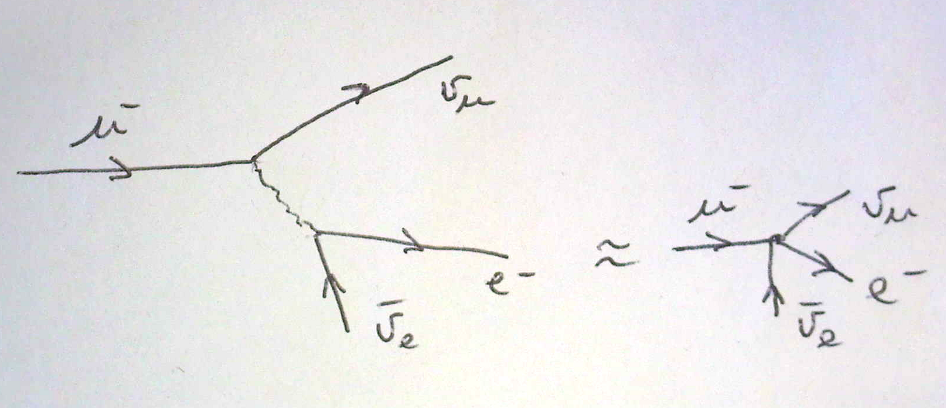
\includegraphics[width=0.75\textwidth]{kap06_01.png}




\[T= \frac{G_F}{\sqrt{2}}\underbrace{  \overline\psi(p_2)\gamma^\mu(1-\gamma_5)\psi(p_1)}_{J^{\text{myon}}} \underbrace{\overline\psi(k_1)\gamma_\mu(1-\gamma_5)\psi(k_2)}_{J^{\text{elektron}}}\]


\(J^{\text{myon}}\cdot J^{\text{elektron}} = \text{Lorenz-Skalar?}\) \(\rightarrow \) Parität:

\begin{align}
T\rightarrow T' &=\frac{G_F}{\sqrt{2}} \overline\psi'(p_2')\gamma^\mu(1-\gamma_5) \psi'(p_1')   \overline\psi'(k_1')\gamma^\mu(1-\gamma_5) \psi'(k_2') \\
&=\frac{G_F}{\sqrt{2}} \overline\psi(p_2)\underbrace{P^{-1}\gamma^\mu(1-\gamma_5)P}_{\gamma^\mu (1+\gamma_5)}  \psi(p_1)   \overline\psi(k_1)\underbrace{P^{-1}\gamma^\mu(1-\gamma_5)P}_{\gamma_\mu (1+\gamma_5)} \psi(k_2) \\
&=\frac{G_F}{\sqrt{2}} \overline\psi(p_2)\gamma^\mu (1+\gamma_5) \psi(p_1)   \overline\psi(k_1)\gamma_\mu (1+\gamma_5) \psi(k_2)\\
 &\neq T\\
\end{align}

\(\beta\)-Zerfall: sehr ähnlich, jedoch Koeffizienten \(c_\mu,c_\lambda\) für Nukleonen


\section{Bedeutung der omega Parameter}

\[S(\Lambda) = e^{-\frac{1}{4}(\omega^{12}\sigma_{12}+\omega^{22}\sigma_{21})}= e^{-\frac{i}{2}\omega^{12}\sigma_{12}}\]

\[\frac{1}{2}\sigma_{12} = \frac{1}{2}\frac{i}{2}[\gamma_1,\gamma_2] = \frac{i}{4}\underbrace{\left[ \begin{pmatrix} 0&-\sigma_1\\   \sigma_1&0 \end{pmatrix}, \begin{pmatrix} 0&-\sigma_2\\   \sigma_2&0 \end{pmatrix} \right]}_{=  \begin{pmatrix} -[\sigma_1,\sigma_2]&0\\  0&- [\sigma_1,\sigma_2] \end{pmatrix}  } =  \begin{pmatrix} \frac{\sigma_3}{2}&0\\0& \frac{\sigma_3}{2} \end{pmatrix} = \frac{S_z}{\hbar} \]


mit \(\gamma_5 = \begin{pmatrix} 0&1\\   1&0 \end{pmatrix} \) allgemeiner:

\[\frac{1}{2}\sum_k = \frac{S_k}{\hbar} = \frac{1}{4} \epsilon^{ijk}\sigma_{ij} = \frac{1}{2} \gamma_5\alpha_k\]

\(\omega_1\) und \(\omega_3\) sind EZ von \(S_z\) zu \(+\frac{\hbar}{2}\); \(\omega_2\) und \(\omega_4\) sind EZ von \(S_z\) zu \(-\frac{\hbar}{2}\);

Jetzt boost in Bezugssystem mit Geschwindigkeit \(\vec v\)

Dazu

\[\omega^{\mu\nu}   =\begin{pmatrix} 0&+n_1&+n_2&+n_3\\  -n_1&0&0&0\\   -n_2&0&0&0\\  -n_3&0&0&0 \end{pmatrix}\vec n^2 = 1 \]

\[ S(\Lambda) = e^{-\frac{i}{4}\omega^{\mu\nu}\sigma_{\mu\nu}}  = e^{-\frac{i}{2}\sum_j\omega^{0j}\sigma_{0j}} = e^{-\frac{1}{2}\omega \vec n\vec \alpha}  \]

mit \( \sum_j\omega^{0j}\sigma_{0j} = \omega \vec n \frac{i}{2}\underbrace{[\beta,-\beta\vec\alpha]}_{-2\vec\alpha} \)

Verschiebung von \(\omega^{\mu\nu}\) und \(\vec v\)


\[\Lambda^\mu_{\,\,\nu}: \qquad \Lambda = \lim_{N \to \infty} (g+\frac{\omega}{N})^N = exp\left\{\omega\underbrace{ \begin{pmatrix} 0&+n_1&+n_2&+n_3\\  -n_1&0&0&0\\   -n_2&0&0&0\\  -n_3&0&0&0 \end{pmatrix}}_{I}  \right\}\]

Spezialfall \(n_1 = 1, n_2=n_3 = 0\)

\[I^2 = \begin{pmatrix} 1&0&0&0\\ 0&1&0&0 \\ 0&0&0&0\\ 0&0&0&0 \end{pmatrix};\qquad I^3=I;\qquad etc. \]

\[\Lambda = e^{\omega I} = cosh(I\omega) + sinh(I\omega) =  \begin{pmatrix} cosh\omega&-sinh\omega&0&0\\ -sinh\omega&cosh\omega&0&0 \\ 0&0&1&0\\ 0&0&0&1 \end{pmatrix} \]

vergleiche \(x^{'\nu} = \Lambda^\nu_{\,\,\mu}x^\mu\)


\[x^{0'} = cosh\omega(x^0-tanh\omega x') = \gamma(ct-\frac{v}{2}x)\]

\[x^{''} = cosh\omega(x'-tanh\omega x^0) = \gamma(x-\frac{v}{2}ct)\]

\[\Rightarrow tanh \omega = \frac{v}{c} = \frac{|\vec p|^2}{E}\]

\[cosh\omega =\gamma = \frac{1}{\sqrt{1-\frac{v^2}{c^2}}} = \frac{E}{m^2} \]


\(\Rightarrow \) Allgemeiner Fall \(\vec n = \hat v\); \(tanh\omega = \frac{v}{c}\)


Rapidität = \(\frac{1}{2} ln\frac{E+|\vec p|c}{E-|\vec p|c} =\frac{1}{2} ln\frac{1+tanh\omega}{1-tanh\omega} = \frac{1}{2} ln\frac{cosh\omega+sinh\omega}{cosh\omega-sinh\omega}  = \frac{1}{2}ln\frac{e^\omega}{e^{-\omega}} =\omega \)


\subsection{Ebene-Wellen-Lösung zu allg. Impuls}

\[(i\cancel \partial - \frac{mc}{\hbar})\psi(x) = 0\]

Lösung mit \(\psi(x) = e^{-i\frac{px}{\hbar}}\omega(\vec p)\)

\(\vec p\) in Ruhe

\[E = +mc^2\qquad \omega_1(0) = \begin{pmatrix} 1\\ 0 \\ 0\\ 0 \end{pmatrix},\qquad \omega_2(0) = \begin{pmatrix} 0\\ 1 \\ 0\\ 0 \end{pmatrix} \]

\[E = -mc^2\qquad \omega_3(0) = \begin{pmatrix} 0\\ 0 \\ 1\\ 0 \end{pmatrix},\qquad  \omega_4(0) = \begin{pmatrix} 0\\ 0 \\ 0\\ 1 \end{pmatrix} \]

Besser für Teilchenwellenfunktionen immer \(E>0\), d.h.

\[p^\mu = (\frac{E}{c},\vec p) = (+\sqrt{m^2c^2+\vec p^2},\vec p)\]

Lsg pos. Energie \(\psi(x) = e^{-i\frac{px}{\hbar}}\omega_i(\vec p)\) mit i=1,2

Lsg neg. Energie \(\psi(x) = e^{+i\frac{px}{\hbar}}\omega_i(\vec p)\) mit i=3,4

\[\Rightarrow (\cancel p -mc) \omega_i(\vec p) = 0 \qquad i=1,2\]

\[\Rightarrow (\cancel p +mc) \omega_i(\vec p) = 0 \qquad i=3,4\]

Jetzt \(\omega_i(\vec p)\) durch boost von \(\omega_i(0)\) entlang der \(\vec p\)- Richtung:

ungestricheltes System = Ruhesystem des Teilchens
gesticheltes System = Teilchen bewegt sich in \(\vec p \)-Richtung

\(\Rightarrow \) boost in \(-\vec p\)-Richtung um Teilchen in Bewegung zu setzen

\[\Rightarrow \omega_\nu(\vec p) = S(\Lambda)\omega_\nu(0) = e^{\frac{1}{2}\omega\hat p\vec\alpha}\omega_\nu(0)  \]

Diese \(\omega_\nu(\vec p)\) ist der Spinor der Elektornen mit Impuls \(\vec p\) und Spin in Ruhesystem in \(\pm z\)-Richtung beschreibt

\[\hat p\vec \alpha = \begin{pmatrix} 0& \hat p\vec\sigma \\ \hat p\vec \sigma& 0 \end{pmatrix} \]

\[ (\hat p\vec \alpha)^2 = \begin{pmatrix} (\hat p\vec\sigma)^2&0 \\0& (\hat p\vec \sigma)^2 \end{pmatrix} =  \begin{pmatrix} \mathbb 1_2&0 \\0& \mathbb 1_2 \end{pmatrix}  \]

\[\Rightarrow e^{\frac{1}{2}\omega\hat p\vec\alpha} = cosh\frac{\omega}{2}\mathbb 1 + sinh(\frac{\omega}{2})(\hat p\vec \alpha)\]

\[cosh\frac{\omega}{2} = \sqrt{\frac{1+cosh\omega}{2}} = \sqrt{\frac{1+E/mc^2}{2}} =  \sqrt{\frac{E+mc^2}{2mc^2}} \]


\[sinh\frac{\omega}{2} = \sqrt{cosh^2\frac{\omega}{2}-1} =  \sqrt{\frac{E-mc^2}{2mc^2}} =  \sqrt{\frac{E+mc^2}{2mc^2} \frac{(E-mc^2)(E+mc^2}{(E+mc^2)} } = \sqrt{\frac{E+mc^2}{2mc^2}} \frac{|\vec p|c}{E+mc^2}   \]

\begin{align}
S(\Lambda) &= e^{\frac{1}{2}\omega\hat p \vec\alpha} = cosh\frac{\omega}{2}(\mathbb 1 + \frac{c\hat p\vec\alpha}{E+mc^2})\\
&=\sqrt{\frac{E+mc^2}{2mc^2}} \begin{pmatrix}1&0&\frac{cp_+}{E+mc^2}&\frac{cp_-}{E+mc^2}\\0&1&\frac{cp_+}{E-mc^2} &-\frac{cp_+}{E+mc^2}\\\frac{cp_z}{E+mc^2} &\frac{c(p_x-ip_y)}{E+mc^2}&1&1\\\frac{c(p_x+ip_y)}{E+mc^2} &-\frac{cp_z}{E+mc^2} &0&1\end{pmatrix} \\
&= (\omega_1(\vec p),\omega_2(\vec p), \omega_3(\vec p),\omega_4(\vec p))
\end{align}

mit \(p_\pm = p_x\pm ip_y\)


\section{Der Diracsee}



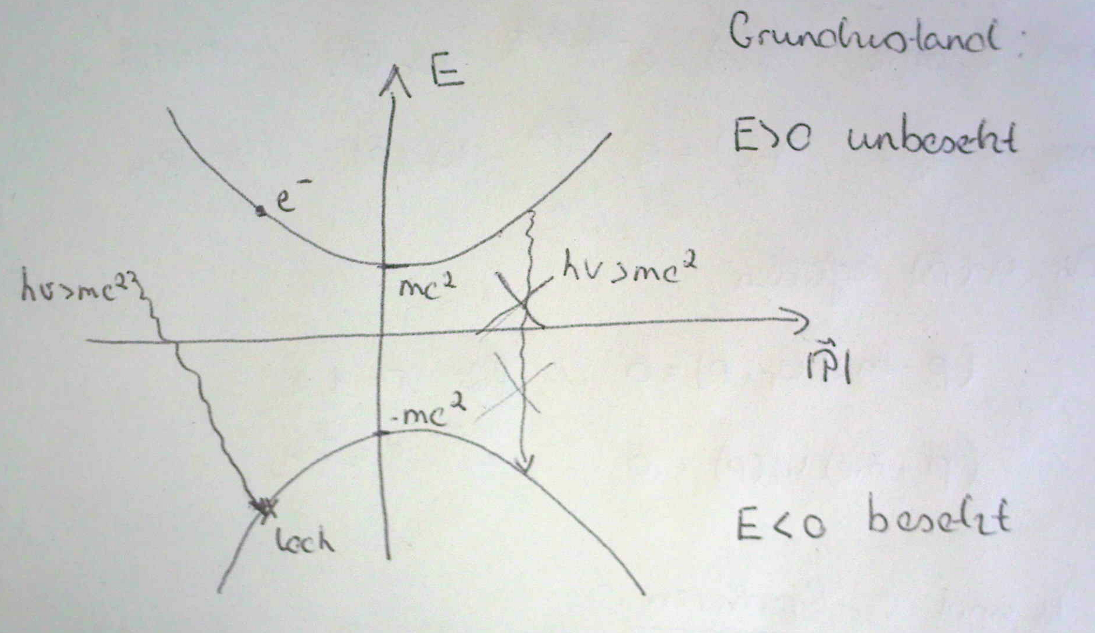
\includegraphics[width=0.75\textwidth]{kap06_02.png}

Grundzustand:

 \(E>0\) unbesetzt

\(E<0\) alle besetzt \(\Rightarrow \) Pauli Prinzip verbietet Übergänge von \(E>0 \rightarrow E<0 \)

Elektron: Zustand mit \(E>mc^2\) , Ladung \(-|e|\), Spin \(S_z\)

Loch: es fehlt Elektron mit \(E<0\)

Gegenüber Grundzustandd: Energieerhöhung um \(-E = +\sqrt{m^2c^4+(\vec pc)^2}\)

Ladung \(+|e|\)
Spin \(-S_z\)

\(\rightarrow \)\underline{Positronen mit positiver Ladung} \(E>0\)

Lösungen der Dirac Gl: \(E=p^0 = +\sqrt{m^2c^4+(\vec pc^2)}\)

pos. Energie: \(\psi(x) = e^{-ipx/\hbar}w_r(\vec p)\) mit \(r=1,2\)

neg. Energie: \(\psi(x) = e^{+ipx/\hbar}w_r(\vec p)\) mit \(r=3,4\)

Die \(w_r(\vec p)\) erfüllen

\[(\cancel p - mc)w_r(\vec p) = 0 \qquad\text{für } r=1,2\]

\[(\cancel p + mc)w_r(\vec p) = 0 \qquad\text{für } r=3,4\]


\underline{u und v Spinoren}


Ruhesystem des \(e^{\pm}\). \(\overline p^\mu = (mc,\vec 0)\) 4 Impuls 

\(\overline S^\mu = (0,\vec S)(\vec s^2=1\)  \(\vec S\) Quant. achse


Boost in IS in dem \(p^0 = +\sqrt{(mc^2)^2+(\vec p c)^2}\quad:\quad \Lambda^\mu_{\,\,\nu} \)

\[p^\mu = \Lambda^\mu_{\,\,\nu}\overline p^\nu, \qquad s^\nu =\Lambda^\mu_{\,\,\nu}\overline s^\nu \]

\[\Rightarrow p^2=m^2c^2, \quad p\cdot s = \overline p\cdot \overline s = 0,\quad s^2 = -1\]

\(e^-:\quad \psi(x) = e^{-ipx/\hbar}u(p,\pm s)\)

\(e^+:\quad \psi(x) = e^{+ipx/\hbar}v(p,\pm s)\)


Für \(\vec S = \hat z\):

Elektron:
\[w_1(\vec p) = u(p,+s)\]
\[w_2(\vec p) = u(p,-s)\]

Positron:
\[w_3(\vec p) = v(p,-s)\]
\[w_4(\vec p) = v(p,+s)\]

Normierung der \(u,v\) \(\epsilon,\epsilon' = \pm 1\)

\[\overline u(p,\epsilon s) u(p,\epsilon' s)\quad ^{L.I.}= \overline u(\overline p,\epsilon\overline s)  u(\overline p,\epsilon'\overline s) = w^+_{r(\epsilon)}(\vec 0)\gamma^0w_{r'(\epsilon')}(0) = \delta_{\epsilon\epsilon'}\]

\[\overline u(p,\epsilon s) v(p,\epsilon' s) = 0\]

\[\overline v(p,\epsilon s) v(p,\epsilon' s) =-\delta_{\epsilon'\epsilon}\qquad \text{wegen} \gamma^0 = \begin{pmatrix}1&0&0&0\\ 0&1&0&0\\0&0&-1&0\\0&0&0&-1\end{pmatrix} \]

\underline{Vollständigkeit}

Jeder Spinor kann als Linearkombination von \(u(p,s), u(p-s), v(p,s), v(p,-s)\) geschrieben werden.

\[\Rightarrow \sum_{\epsilon'} u_{A}(p,\epsilon's )\overline u_B(p,\epsilon' s) = \left(\frac{\cancel p +mc}{2mc}\right)_{AB} = (\Lambda_+(p))_{AB}\]

Bew: Angewendet auf \(u,v\) Spinoren, geben beide Matrizen gleiches Ergebnis

\[\frac{\cancel p + mc}{2mc} u(p,\epsilon s) =\frac{\cancel p -mc+2mc}{2mc} u(p,\epsilon s) = u(p,\epsilon s) \]


\[\frac{\cancel p + mc}{2mc} v(p,\epsilon s) = 0 \]


Andererseits

\[\sum_{\epsilon'} u(p,\epsilon' s)\underbrace{\overline u(p,\epsilon s) u(p,\epsilon s)}_{\delta_{\epsilon'\epsilon}} = u(p,\epsilon s)\]

\[\sum_{\epsilon} u(p,\epsilon' s)\underbrace{\overline u(p,\epsilon' s) v(p,\epsilon s)}_{=0} = 0\]


Analog für \(v\) Spinoren

\[ \sum_{\epsilon'} u_A(p,\epsilon' s) \overline u_B(p,\epsilon' s) = \left(\frac{\cancel p -mc}{2mc}\right)_{AB}\]


denn \(\sum_{\epsilon'} v(p,\epsilon' s)\underbrace{\overline v (p,\epsilon' s) v(p,\epsilon s)}_{-\delta_{\epsilon'\epsilon}} = -v(p,\epsilon s)\)

\[ \left(\frac{\overbrace{\cancel p}^{-mc} -mc}{2mc}\right) v(p,\epsilon s) = -v(p,\epsilon s) \]


\(\Lambda_+(p)\) ist Projektor auf Zustände pos. Energie \(e^-\)

\(\Lambda_-(p)\) ist Projektor auf Zustände neg. Energie \(e^+\)

Beweis: z.Z: \(\Lambda^2_{\pm}=\Lambda_\mp,\quad \Lambda_+\Lambda_- = 0,\quad \Lambda_++\Lambda_- = \mathbb 1\) mit \(\cancel p^2 = p^2\)

\[ \Lambda_{\pm} = \frac{mc\pm \cancel p}{2mc} \Rightarrow \Lambda^2_{\pm} = \frac{m^2c^2\pm 2mc\cancel p+p^2}{(2mc)^2} = 2mc \frac{mc\pm \cancel p}{(2mc)^2} = \Lambda_\pm\]


\[ \Lambda_+\Lambda_- = \frac{mc+\cancel p}{2mc}\frac{mc-\cancel p}{2mc} = \frac{(mc)^2-p^2}{(2mc)^2} = 0 \]

\[ \Lambda_++\Lambda_- = = \frac{mc+\cancel p + mc - \cancel p}{2mc} = \mathbb 1 \]


\section{Ladungskonjugation}

Dirac Gl. sollte auch für Positronen als Teilchen , Elektronen als Antiteilchen existieren. (mit Spinor \(\psi_C\))

\[(i\hbar \cancel \partial\underbrace{+e\cancel A}_{-q_e+\cancel A}-mc)\psi_C(x) = 0\]

(e<0 = Ladungsvorzeichen \(e^-)\)

Ges. Beziehung zur Dirac Gl. für \(e^-\)

\[ i\hbar\cancel \partial - e\cancel A - mc)\psi(x) = 0 \]

\[\Rightarrow [-(i\hbar\partial_\mu+eA_\mu)\gamma^{*\mu} - mc]\psi^*(x) = 0\qquad |\cdot C\gamma^0\]

Transformation mit Matrix \(C\gamma^0\)

\[\Rightarrow  [(i\hbar\partial_\mu+eA_\mu)(-C\gamma^0\gamma^{*\mu}((\gamma^0)^{-1} - mc]C\gamma^0\psi^*(x) = 0  \]


gesucht \(C\) mit \( C\gamma^0\gamma^{*\mu} (C\gamma^0)^{-1} = -\gamma^\mu\) !

Dann ist \(\psi_C (x) = C\gamma^0\psi^*(x) = C(\gamma^0)^T(\psi^\dagger)^T = C(\psi^\dagger\gamma^0)^T = C\overline \psi^T(x)\)

die Matrix \(C=i\gamma^2\gamma^0\) tut's !

\[\Rightarrow C\gamma^0 = i\gamma^2\gamma^0\gamma^0 = i\gamma^2 = (C\gamma^0)^{-1},\qquad (\gamma^2)^2 = -\mathbb 1, \quad (i\gamma^2)^2 = +\mathbb 1\]

\[C\gamma^0(\gamma^\mu)^*(C\gamma^0)^{-1} = i\gamma^2\gamma^{*\mu}i\gamma^2 = -\gamma^2\gamma^{\mu*}\gamma^2 = \begin{cases}
  \mu = 2:  & -\gamma^2(-\gamma^2)\gamma^2 = -\gamma^2\\
  \text{sonst }&-\gamma^2\underbrace{\gamma^\mu\gamma^2}_{-\gamma^2\gamma^\mu} = -\gamma^\mu
\end{cases}\]

Es gilt auch

\[C\overline u^T (p,s) = v(p,s) \cdot e^{i\alpha}\]

\[C\overline v^T (p,s) = u(p,s) \cdot e^{i\alpha'}\]

\end{document}